\def \delta {0.15}

\begin{tikzpicture}
\tikzstyle{task} = [draw, fill=white,align=center]

%%%%%%%%%%%
%%% CPS %%%
%%%%%%%%%%%

%%% TASKS %%%

\node[task,] (t1) at (-2+0*\delta,1.6-0*\delta) {Task $\#1$ \\\faFileCode[regular]};
\node[task,] (t2) at (-2+1*\delta,1.6-1*\delta) {Task $\#2$ \\\faFileCode[regular]};
\node[task,] (t3) at (-2+2*\delta,1.6-2*\delta) {Task $\#3$ \\\faFileCode[regular]};

\node[task,] (ct1) at (1+0*\delta,1.6-0*\delta) {Control-Task $\#1$ \\\faFileCode[regular]};
\node[task,] (ct2) at (1+1*\delta,1.6-1*\delta) {Control-Task $\#2$ \\\faFileCode[regular]};
\node[task,] (ct3) at (1+2*\delta,1.6-2*\delta) {Control-Task $\#3$ \\\faFileCode[regular]};

%%% CYBER %%%

\node[align=center] (rtos) at (-0.2,0.15)  {Real-Time Operating System};
{\color{lqgcolour}\node[draw, align=center, rotate=90, text width=3.0cm] (hw)   at (3.35,0.775) {HW interfaces};}
\node[fit=(rtos)(t1)(ct1)(ct3),draw,yshift=1.5mm] (sw) {};
\node[draw, above left] (clock) at (sw.south east)  {\faClock[regular]};
\node[thick, fit=(sw)(hw),draw] (board) {};
\node[above left, xshift=1.8cm] (borad-label) at (board.south west) {Board};
\node[draw, above right] (clockboard) at (board.south west)  {\faClock[regular]};

%%% PHYSICAL %%%

\node[thick, draw ,align=center] (phys) at (6,0.775) {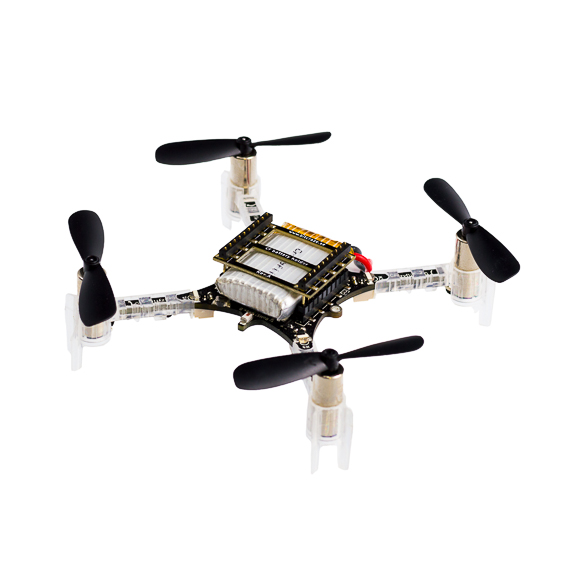
\includegraphics[scale=0.4]{figs/topic/crazyflie.jpg}};
\node[draw, above left] (time) at (phys.south east)  {\faClock[regular]};

%%% ARROWS %%%

\draw[-latex] ([yshift=0.65cm]hw.south) to node[yshift=0.85cm,rotate=90]{actuation} ([yshift=0.65cm]phys.west);
\draw[-latex] ([yshift=-0.65cm]phys.west) to node[yshift=-0.85cm, rotate=90]{sensing} ([yshift=-0.65cm]hw.south);

\end{tikzpicture}
